\documentclass[a4paper]{scrartcl}
\usepackage[latin1]{inputenc}			% Für Umlaute
\usepackage[T1]{fontenc}			% Für richtige Schrift
\usepackage[ngerman]{babel}			% Für neue deutsche Rechtschreibung (Trennung)
\usepackage{color}
\usepackage{amsmath}
\usepackage{amssymb}
\usepackage{graphicx}
\usepackage{textcomp}				% Fürs Gardzeichen

\usepackage{scrpage2}				% Für Kopf- und Fußzeilen
\pagestyle{scrheadings}				% Für Kopf- und Fußzeilen
\clearscrheadfoot					% Für Kopf- und Fußzeilen

\renewcommand{\labelenumi}{(\alph{enumi})}
\renewcommand{\labelenumii}{(\roman{enumii})}

\begin{document}
\titlehead{Wintersemester 2017/2018\\Motion Planning\\Prof. Horsch, Rudi Scheitler}
\author{David Welsch, Ken Hasenbank}
\title{Praktikum 5 - Rapidly Exploring Random Trees (RRT)}
\maketitle

\section*{Beschreibung der Aufgabe}

Das Ziel dieses Praktikums war es, auf Basis eines RRT's einen Weg zwischen einer Start- und einer Zielkonfiguration zu finden. \\

Das Konzept von RRT's ist es, eine zufällige Konfiguration an den bissherigen RRT anzuschließen. Hierfür wird der Punkt auf dem Graphen gesucht, der der neuen zufälligen Konfiguration am nächsten ist. Nun wird von dem gefundenen Punkt aus in Richtung der neuen Konfiguration gegangen und - vorrausgesetzt es wurde kein Hindernis getroffen - der entsprechende Weg als Edge in den Graphen gespeichert. Wird jedoch ein Hindernis getroffen kann der Weg auch nur zu Teilen in den Graphen aufgenommen werden, um so nah wie möglich an den Rand des Hindernisses heran zu kommen. Kann man anstelle der zufälligen Konfiguration die Zielkonfiguration direkt an den RRT anschließen kann das "exploring" beendet werden und über einen Graph-Such-Algorithmus wie beispielsweise dem A* oder Dijkstra ein Pfad zwischen der Start- zu Zielkonfiguration gefunden werden.\\

In den gegebenen Aufgaben soll zunächst ein simpler, zweidimensionaler RRT im Einheitsquadrat ohne Hindernisse generiert werden. Danach soll ein Wurm mit 5 Freiheitsgraden (zwei davon translatorisch, drei rotatorisch), wie auch schon im \textit{Praktikum 4}, durch einen Parcours mit 5 Hindernissen bewegt werden.

\section*{Beschreibung der L"osung}

Zur L"osung haben wir den Code-Rahmen des PRM-Praktikums verwendet und um die Funktion des Tools GnuPlot erweitert. Alle Berechnungen erfolgen in der Datei \textit{main.cpp} und dort in der Methode \textit{\_tmain}. Wir nutzen zudem eine Methode um die Kanten zum Graphen hinzuzufügen.\\

Ab hier wird durch die Beschreibung der Datei \textit{main.cpp} unser Vorgehen erläutert:

Zunächst sind sowohl die Aufgabe 1 als auch die Aufgabe 2 (inklusive des freiwilligen Teils) in einem Projekt. Zwischen den Aufgaben kann über einen define in Zeile 236 \textit{define AUFGABE 1|2} gewechselt werden. 

\begin{itemize}
	\item Aufgabe 1 (Zeilen 233 - 320)
		Zur Lösung dieser Aufgabe mussten wir den vorgegebenen Coderahmen zunächst so umbauen, dass er einfache 2-dimensionale Konfigurationen entgegen nimmt. Anschließend haben wir als initiale Konfiguration den Mittelpunkt \textit{\{0.5, 0.5\}} in den Graphen aufgenommen. Anschließend generieren wir mittels eines Zufallsgenerators zufällige Konfigurationen und suchen unter Zuhilfenahme eines rTrees den nächsten Punkt auf dem Graphen um diese beiden Punkte dann miteinander zu verbinden. Die Punkte werden allerdings nicht direkt verbunden sondern in einer kleinen Schrittgröße zerstückelt. Dieser Vorgang wird 1000 mal wiederholt (definiert in Zeile 238), wobei alle 10\% der aktuelle Graph in eine GnuPlot-Datei abgespeichert wird. Die Zwischenschritte können, wie in Abbildung \ref{inter} zu sehen, über das Tool GnuPlot gerendert werden.
		\begin{figure}[h!]
			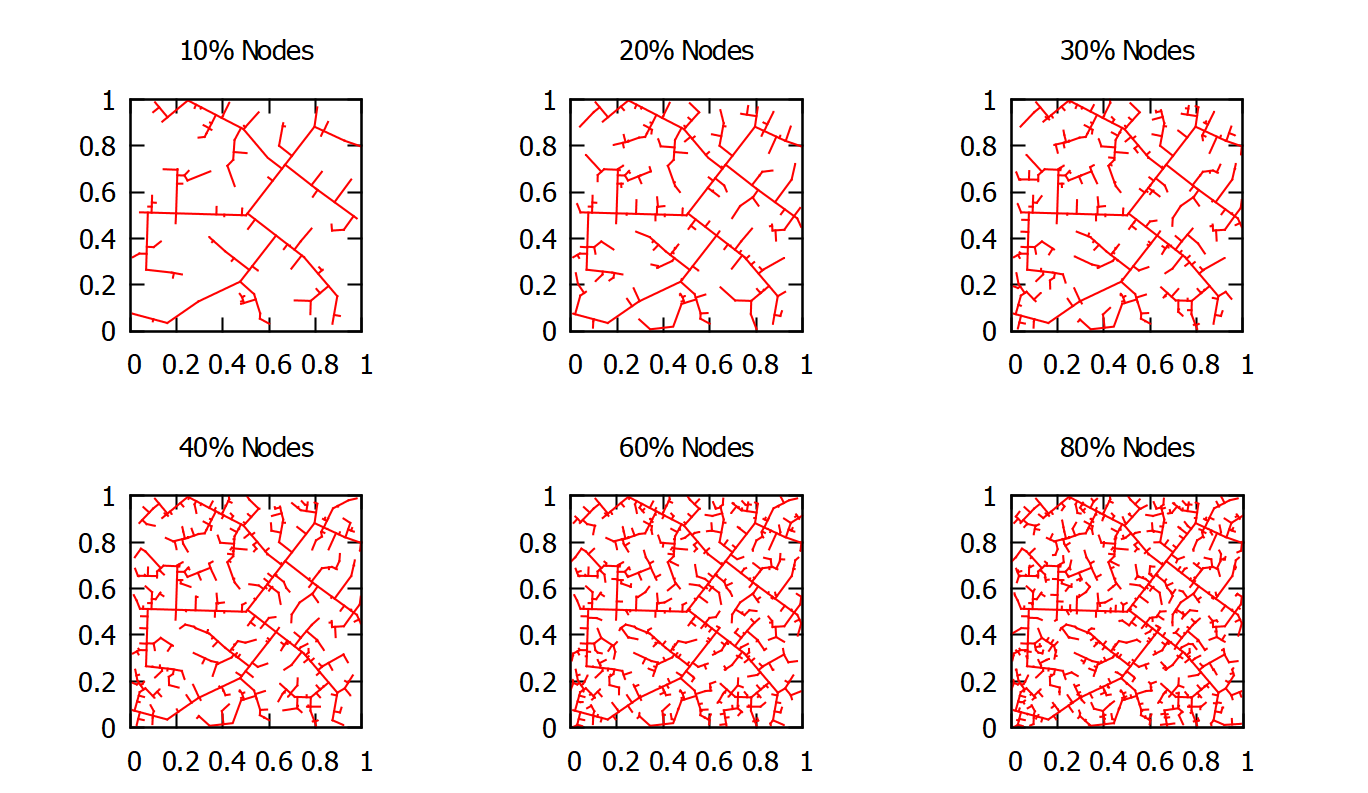
\includegraphics[width=\textwidth]{inter.png}
			\caption{Zwischenschritte}
			\label{inter}
		\end{figure}
		In Abbildung \ref{inter} ist gut zu erkennen, dass der Baum den gesamten Raum sehr schnell erkundet und anschließend nur noch feinkundiger untersucht. So sieht man in den ersten 50\% die größten Unterschiede zwischen den einzelnen stufen. Darüber hinaus wird der Graph nur noch um sehr kurze Verzweigungen erweitert. Abbildung \ref{full} zeigt nochmal das Ergebnis nachdem alle 1000 Nodes hinzugefügt wurden.
		\begin{figure}[h!]
			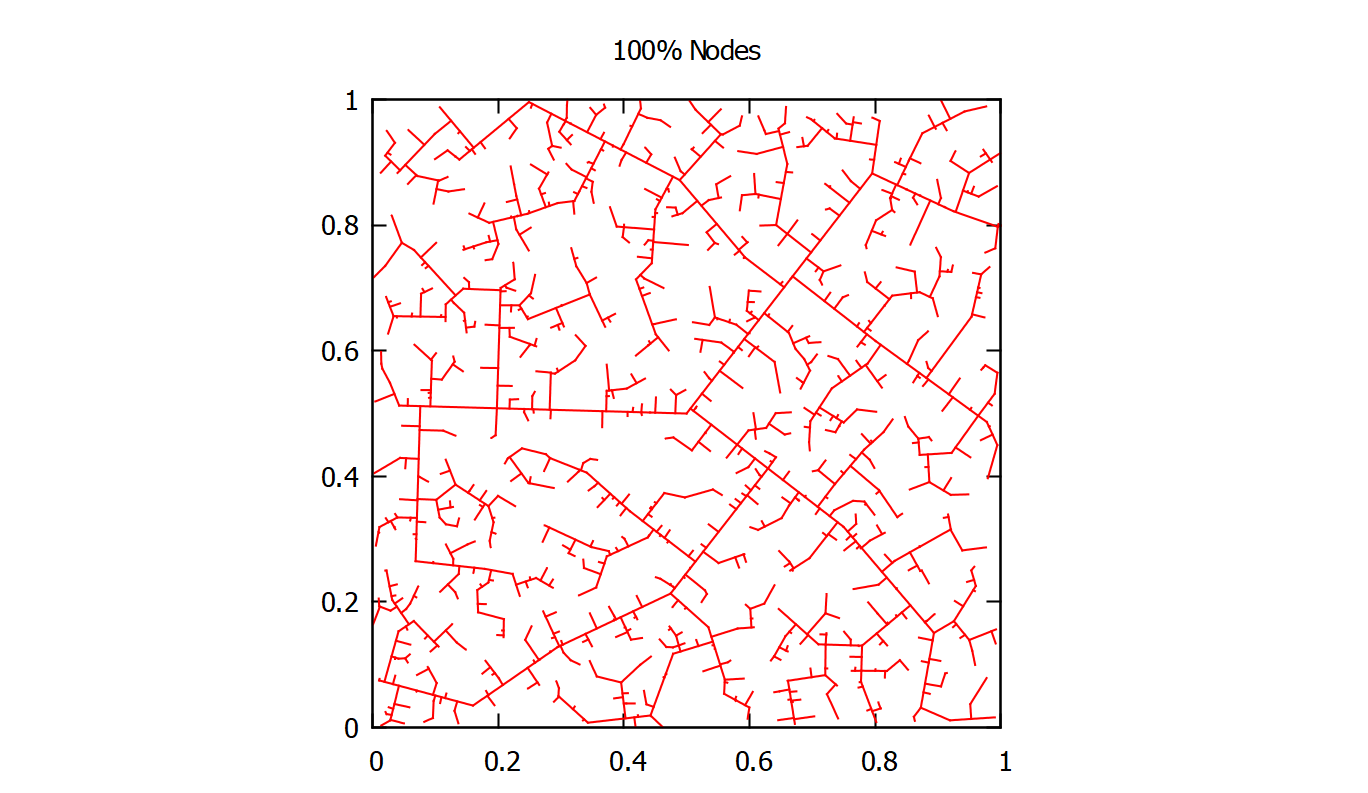
\includegraphics[width=\textwidth]{full.png}
			\caption{Endergebnis}
			\label{full}
		\end{figure}
	\item Aufgabe 2 (Zeilen 102 - 223 und 322 - 567)
	\begin{itemize}
		\item Funktionen (Zeilen 102 - 223)
		\begin{itemize}
			\item \textit{getVector} \\
				Diese Funktion gibt die Konfiguration einer angegebenen Position aus einem Graphen zurück.
			\item \textit{addVertex} \\
				Diese Funktion fügt eine Konfiguration in zwei unabhängigen Graphen und den dazugehörenden rTrees hinzu. Dies wird verwendet um zwei separate Graphen für Start- und Zielkonfiguration pflegen zu können und trotzdem am Ende alle Daten in einem globalen Graphen vorliegen zu haben.
			\item \textit{findNearest} \\
				Sucht mittels eines rTrees die \textit{n} nächsten Nachbarn zu einem angegebenen Punkt aus einem Graphen und gibt diese zurück.
			\item \textit{doStep} \\
				Diese Funktion geht, von einen gegebenen Startkonfiguration, eine Schrittlänge entgegen der angegebenen Zielkonfiguration. Ist die Entfernung zwischen der Start-/ und Zielkonfiguration geringer als die angegebene Schrittlänge wird die Zielkonfiguration zurück gegeben.
			\item \textit{exploreRandom} \\
				Diese Funktion wird verwendet um einen Graphen um eine zufällige Konfiguration zu erweitern.\\
				Es wird zunächst eine zufällige Konfiguration im Konfigurationsraum erzeugt (unabhängig ob diese im Freiraum liegt oder nicht). Anschließend wird auf dem Graphen der Punkt gesucht welcher der zufälligen Konfiguration am nächsten ist. Von diesem Punkt aus wird eine Schrittweite der zufälligen Konfiguration entgegen gegangen. Ist die neu entstandene Konfiguration im Freiraum und von dem Graphen ohne Kollision auf direktem Wege zu erreichen, so wird der Punkt sowie eine Kante in den Graphen eingefügt.
			\item \textit{expandTowards} \\
				Diese Funktion wird verwendet um einen Graphen in Richtung einer angegebenen Zielkonfiguration zu erweitern.\\
				Dabei wird auf dem Graphen nach der Konfiguration gesucht, welche der Zielkonfiguration am nächsten ist. Von dieser wird schrittweise der Zielkonfiguration entgegen gegangen. Jeder Schritt, der kollisionsfrei durchgeführt werden kann, wird als Punkt und als Kante in den Graphen aufgenommen. Wird die Zielkonfiguration erreicht, wird dies mit dem Rückgabewert \textit{true} an den Aufrufer signalisiert. Bei einer Kollision hingegen wird mit dem Rückgabewert \textit{false} signalisiert, dass der Graph den Zielpunkt nicht erreichen konnte.
		\end{itemize}
		\item Implementierung des Algorithmus (Zeilen 322 - 567)\\
			Der Ablauf des Algorithmus kann mittels der oben beschriebenen Funktionen sehr einfach implementiert werden. Zu Beginn werden die Start-/ sowie Zielkonfigurationen in die entsprechenden Graphen eingetragen. Die folgenden 4 Schritte werden nun solange wiederholt bis die Ziel-/ und Startgraphen verbunden sind (die Graphen sind verbunden wenn der Start-/ oder Zielgraph eine Konfiguration des anderen erfolgreich erreichen konnte):
			\begin{itemize}
				\item Erweitere den Zielgraphen um eine zufällige Konfiguration.
				\item Versuche die hinzugefügte Konfiguration vom Startgraphen aus zu erreichen.
				\item Erweitere den Startgraphen um eine zufällige Konfiguration.
				\item Versuche die hinzugefügte Konfiguration vom Zielgraphen aus zu erreichen.
			\end{itemize}
			Anschließend wird der Graph-Such-Algorithmus Dijkstra auf unseren globalen Graphen (beinhaltet sowohl den Start-/ als auch den Zielgraphen) angewendet und das gefundene Ergebnis in einer EasyRob-Datei ausgegeben.
	\end{itemize}
\end{itemize}

	
\section*{Was wir gelernt haben}

 Wir haben durch Aufgabe 1 schnell gemerkt wie gut der RRT einen Raum erkunden kann und uns dazu entschieden auf die erhöhte Komplexität der Parallelisierung (wie in Praktikum 4 verwendet) zu verzichten. Nachdem wir unseren Code währende der Entwicklung mehrmals getestet haben ist uns schnell klar geworden, dass dies eine gute Entscheidung war. Nach erfolgreicher Implementierung und Testens der angegebenen Start-/ und Zielkonfigurationen (alle Ergebnisse unter 3 Sekunden) waren wir sehr erstaunt, wie viel schneller ein zielgerichteter Algorithmus wie der RRT doch sein kann.

\end{document}